\documentclass{article}

\usepackage[top=0.5in, bottom=0.5in, left=1in, right=1in]{geometry}

\thispagestyle{empty}

\usepackage{tikz}
\usetikzlibrary{decorations.text,decorations.pathreplacing,positioning,chains}

\begin{document}

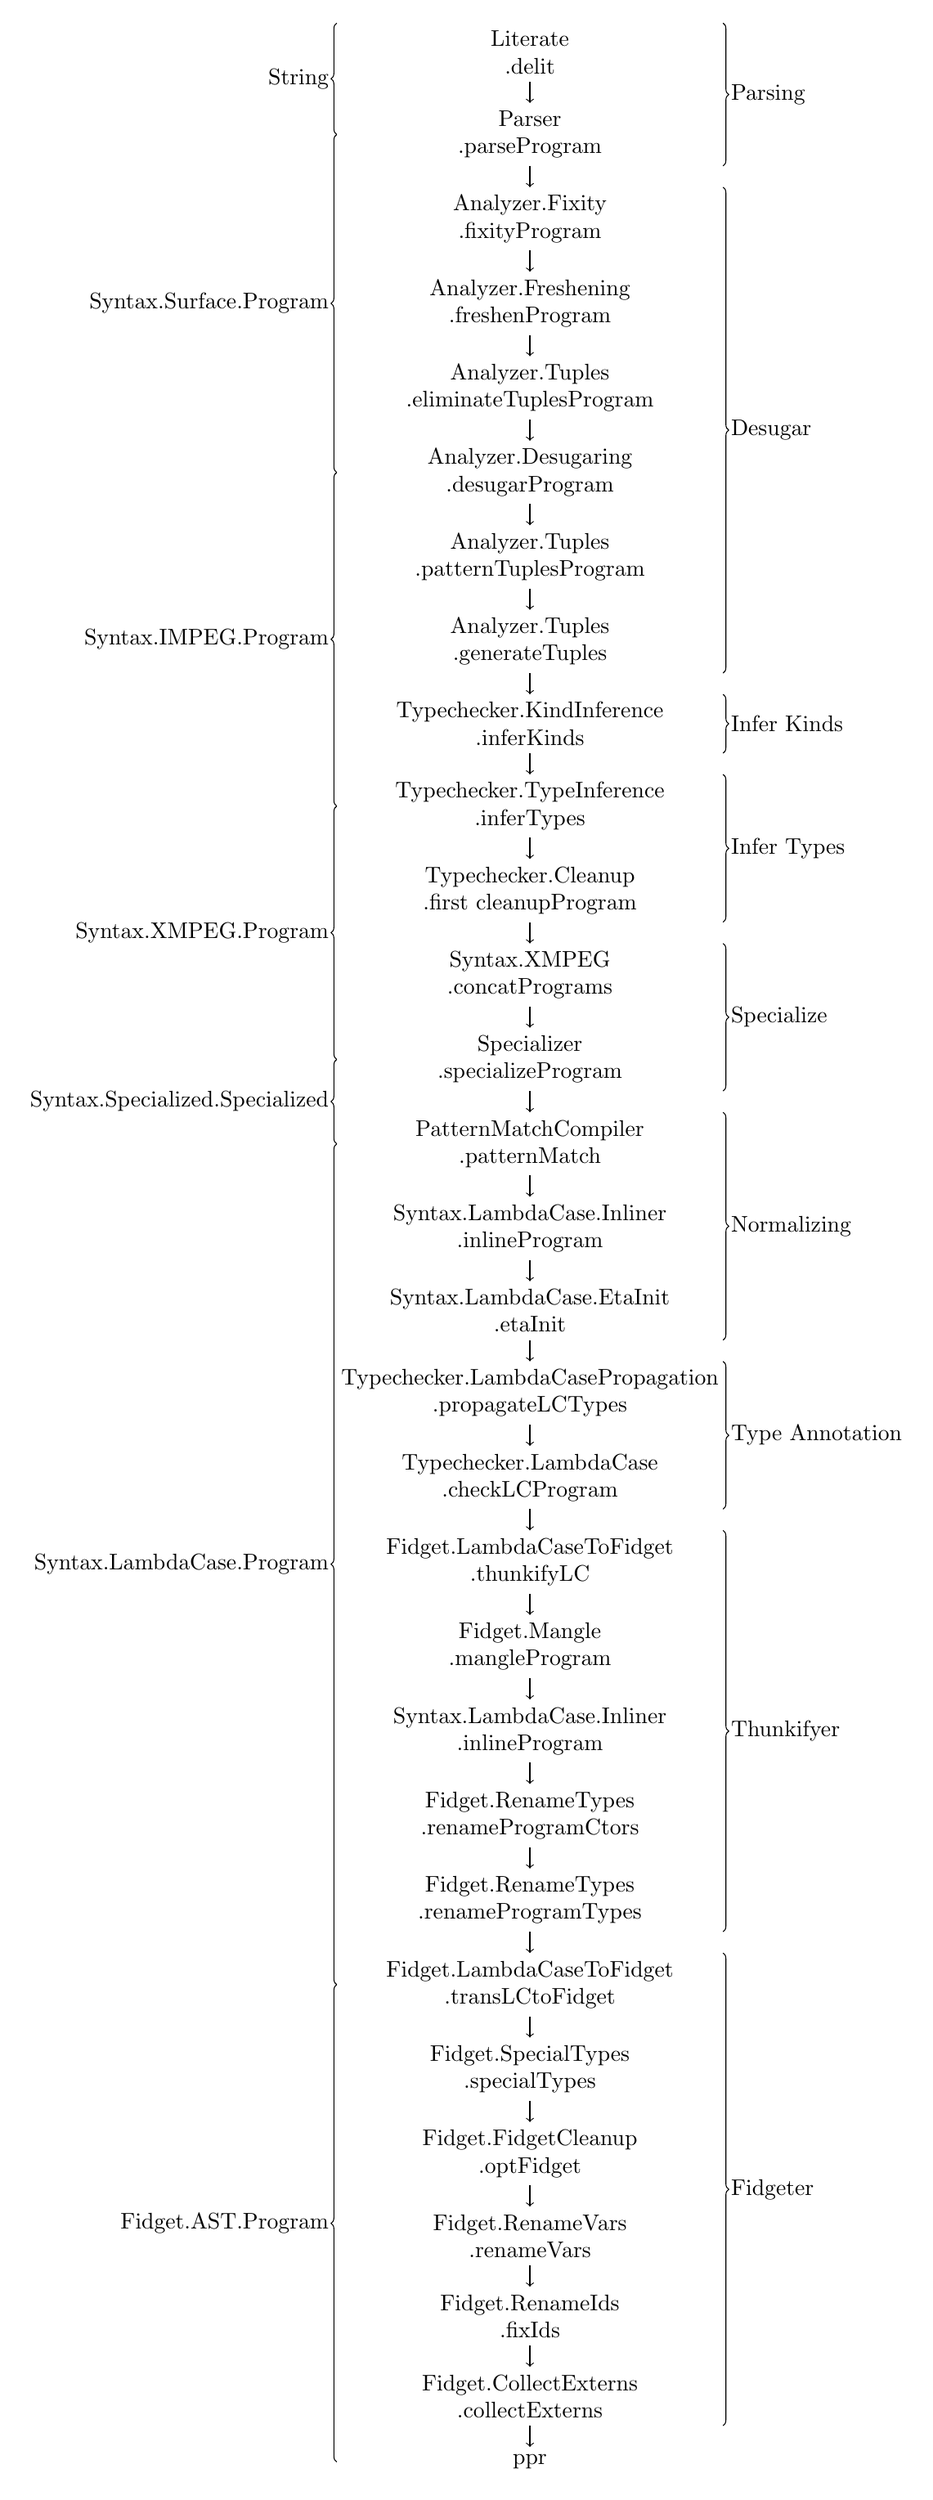
\begin{tikzpicture}

\begin{scope}[start chain=going below,every node/.style={on chain,join},text width=10cm,text centered,node distance=0.33cm,every join/.style=->]
% Parsing
\node (delit) {Literate\\.delit};
\node (parseProgram) {Parser\\.parseProgram};
% toDesugar
\node (fixityProgram) {Analyzer.Fixity\\.fixityProgram};
\node (freshenProgram) {Analyzer.Freshening\\.freshenProgram};
\node (eliminateTuplesProgram) {Analyzer.Tuples\\.eliminateTuplesProgram};
\node (desugarProgram) {Analyzer.Desugaring\\.desugarProgram};
\node (patternTuplesProgram) {Analyzer.Tuples\\.patternTuplesProgram};
\node (generateTuples) {Analyzer.Tuples\\.generateTuples};
% toInferKinds
\node (inferKinds) {Typechecker.KindInference\\.inferKinds};
% toInferTypes
\node (inferTypes) {Typechecker.TypeInference\\.inferTypes};
\node (cleanupProgram) {Typechecker.Cleanup\\.first cleanupProgram};
% toSpecialized
\node (concatPrograms) {Syntax.XMPEG\\.concatPrograms};
\node (specializeProgram) {Specializer\\.specializeProgram};
% toNormalized
\node (patternMatch) {PatternMatchCompiler\\.patternMatch};
\node (inlineProg) {Syntax.LambdaCase.Inliner\\.inlineProgram};
\node (etaInit) {Syntax.LambdaCase.EtaInit\\.etaInit};
% toAnnotated
\node (propagateLambdaCaseTypes) {Typechecker.LambdaCasePropagation\\.propagateLCTypes};
\node (checkLambdaCaseProgram) {Typechecker.LambdaCase\\.checkLCProgram};
% toThunkified
\node (thunkifyLC) {Fidget.LambdaCaseToFidget\\.thunkifyLC};
\node (mangleProgram) {Fidget.Mangle\\.mangleProgram};
\node (inlineProg2) {Syntax.LambdaCase.Inliner\\.inlineProgram};
\node (renameProgramCtors) {Fidget.RenameTypes\\.renameProgramCtors};
\node (renameProgramTypes) {Fidget.RenameTypes\\.renameProgramTypes};
% toFidgetted
\node (transLCtoFidget) {Fidget.LambdaCaseToFidget\\.transLCtoFidget};
\node (specialTypes) {Fidget.SpecialTypes\\.specialTypes};
\node (optimizeFidget) {Fidget.FidgetCleanup\\.optFidget};
\node (renameVars) {Fidget.RenameVars\\.renameVars};
\node (fixIds) {Fidget.RenameIds\\.fixIds};
\node (collectExterns) {Fidget.CollectExterns\\.collectExterns};
% printing
\node (ppr) {ppr};
\end{scope}

\begin{scope}[decoration={brace,raise=3cm},every path/.style={draw,decorate},every node/.style={anchor=west,xshift=3cm}]
\path (delit.north) -- node{Parsing}(parseProgram.south);
\path (fixityProgram.north) -- node{Desugar} (generateTuples.south);
\path (inferKinds.north) -- node{Infer Kinds} (inferKinds.south);
\path (inferTypes.north) -- node{Infer Types} (cleanupProgram.south);
\path (concatPrograms.north) -- node{Specialize} (specializeProgram.south);
\path (patternMatch.north) -- node{Normalizing} (etaInit.south);
\path (propagateLambdaCaseTypes.north) -- node{Type Annotation} (checkLambdaCaseProgram.south);
\path (thunkifyLC.north) -- node{Thunkifyer} (renameProgramTypes.south);
\path (transLCtoFidget.north) -- node{Fidgeter} (collectExterns.south);
\end{scope}

\begin{scope}[decoration={brace,raise=3cm,mirror},every path/.style={draw,decorate},every node/.style={anchor=east,xshift=-3cm}]
\path (delit.north) -- node{String}(parseProgram.center);
\path (parseProgram.center) -- node{Syntax.Surface.Program} (desugarProgram.center);
\path (desugarProgram.center) -- node{Syntax.IMPEG.Program} (inferTypes.center);
\path (inferTypes.center) -- node{Syntax.XMPEG.Program} (specializeProgram.center);
\path (specializeProgram.center) -- node{Syntax.Specialized.Specialized} (patternMatch.center);
\path (patternMatch.center) -- node{Syntax.LambdaCase.Program} (transLCtoFidget.center);
\path (transLCtoFidget.center) -- node{Fidget.AST.Program} (ppr.center);
\end{scope}

\end{tikzpicture}

\begin{tikzpicture}

%\begin{scope}[parent anchor=east,child anchor=west,grow=east]%[start chain=going below,main/.style={on chain,join},text width=10cm,text centered,node distance=0.33cm,every join/.style=->,grow=east]
%\end{scope}

%\end{tikzpicture}

\begin{scope}[parent anchor=east,child anchor=west,grow=east,level distance=8cm,
start chain=going below,main/.style={on chain,join,text width=10cm,text centered},node distance=0.33cm,every join/.style=->]
\node[main] (fidget) {FidgetTypechecker\\.tc\_program\_is\_typed}
%  child { node {tc\_functenv\_of\_functs} }
%  child { node {tc\_functions\_well\_types} }
%  child { node {tc\_programs\_has\_main} }
%  child { node {tc\_init\_is\_valid} }
;
\node[main] (gcminor) {Fidget\_to\_GCminor\\.gcminor\_program}
%  child { node {ids\_noprepet toplevel\_names} }
%  child { node {mk\_liftinfo} }
%  child { node {gen\_tconenv} }
%  child { node {mk\_area\_defn} }
%  child { node {gcminor\_fundefs} }
%  child { node { mk\_new\_main\_fun} }
;
\node[main] {add\_new\_globals\_GCminor};
\node[main] (lowgcminor) {GCminor\_to\_LowGCminor\\.transf\_program};
\node[main] (cminor) {LowGCminor\_to\_Cminor\\.transf\_program};
\end{scope}

\begin{scope}[decoration={brace,raise=3cm,mirror},every path/.style={draw,decorate},every node/.style={anchor=east,xshift=-3cm}]
\path (fidget.north) -- node{Fidget.program}(gcminor.center);
\path (gcminor.center) -- node{GCminor.program} (lowgcminor.center);
\path (lowgcminor.center) -- node{LowGCminor.program} (cminor.center);
\path (cminor.center) -- node{Cminor.program} (cminor.south);
\end{scope}

\end{tikzpicture}

TODO: Parser, GC collector, Interpreter

\end{document}
